% Options for packages loaded elsewhere
\PassOptionsToPackage{unicode}{hyperref}
\PassOptionsToPackage{hyphens}{url}
\PassOptionsToPackage{dvipsnames,svgnames,x11names}{xcolor}
%
\documentclass[
  12pt,
  letterpaper,
]{article}

\usepackage{amsmath,amssymb}
\usepackage{iftex}
\ifPDFTeX
  \usepackage[T1]{fontenc}
  \usepackage[utf8]{inputenc}
  \usepackage{textcomp} % provide euro and other symbols
\else % if luatex or xetex
  \usepackage{unicode-math}
  \defaultfontfeatures{Scale=MatchLowercase}
  \defaultfontfeatures[\rmfamily]{Ligatures=TeX,Scale=1}
\fi
\usepackage{lmodern}
\ifPDFTeX\else  
    % xetex/luatex font selection
\fi
% Use upquote if available, for straight quotes in verbatim environments
\IfFileExists{upquote.sty}{\usepackage{upquote}}{}
\IfFileExists{microtype.sty}{% use microtype if available
  \usepackage[]{microtype}
  \UseMicrotypeSet[protrusion]{basicmath} % disable protrusion for tt fonts
}{}
\usepackage{xcolor}
\usepackage[top=1in,bottom=1in,left=1in,right=1in]{geometry}
\setlength{\emergencystretch}{3em} % prevent overfull lines
\setcounter{secnumdepth}{-\maxdimen} % remove section numbering
% Make \paragraph and \subparagraph free-standing
\ifx\paragraph\undefined\else
  \let\oldparagraph\paragraph
  \renewcommand{\paragraph}[1]{\oldparagraph{#1}\mbox{}}
\fi
\ifx\subparagraph\undefined\else
  \let\oldsubparagraph\subparagraph
  \renewcommand{\subparagraph}[1]{\oldsubparagraph{#1}\mbox{}}
\fi


\providecommand{\tightlist}{%
  \setlength{\itemsep}{0pt}\setlength{\parskip}{0pt}}\usepackage{longtable,booktabs,array}
\usepackage{calc} % for calculating minipage widths
% Correct order of tables after \paragraph or \subparagraph
\usepackage{etoolbox}
\makeatletter
\patchcmd\longtable{\par}{\if@noskipsec\mbox{}\fi\par}{}{}
\makeatother
% Allow footnotes in longtable head/foot
\IfFileExists{footnotehyper.sty}{\usepackage{footnotehyper}}{\usepackage{footnote}}
\makesavenoteenv{longtable}
\usepackage{graphicx}
\makeatletter
\def\maxwidth{\ifdim\Gin@nat@width>\linewidth\linewidth\else\Gin@nat@width\fi}
\def\maxheight{\ifdim\Gin@nat@height>\textheight\textheight\else\Gin@nat@height\fi}
\makeatother
% Scale images if necessary, so that they will not overflow the page
% margins by default, and it is still possible to overwrite the defaults
% using explicit options in \includegraphics[width, height, ...]{}
\setkeys{Gin}{width=\maxwidth,height=\maxheight,keepaspectratio}
% Set default figure placement to htbp
\makeatletter
\def\fps@figure{htbp}
\makeatother

%-----------------------------------------------------------------------------%
%                            SOME PREAMBLE STUFF                              %
%-----------------------------------------------------------------------------%

%-----------------------------------------------------------------------------%
%                            LOAD PACKAGES                                    %
%-----------------------------------------------------------------------------%

\usepackage{hyperref}
\usepackage{setspace}
\usepackage{geometry}
\usepackage[style=apa, backend=biber,annotation=false]{biblatex}
\usepackage[x11names]{xcolor}
\usepackage{longtable}
\usepackage{fancyhdr} % for header
\usepackage{soul} % to make highlight for tags
\usepackage{pdfpages} % to append pdf pages
\usepackage{fontspec} % for fonts

%-----------------------------------------------------------------------------%
%                            Header                                           %
%-----------------------------------------------------------------------------%

\setlength{\headheight}{38pt}
\setmainfont{Helvetica Neue}
\usepackage{booktabs}
\usepackage{caption}
\usepackage{longtable}
\usepackage{colortbl}
\usepackage{array}
\usepackage{anyfontsize}
\usepackage{multirow}
\makeatletter
\@ifpackageloaded{caption}{}{\usepackage{caption}}
\AtBeginDocument{%
\ifdefined\contentsname
  \renewcommand*\contentsname{Table of contents}
\else
  \newcommand\contentsname{Table of contents}
\fi
\ifdefined\listfigurename
  \renewcommand*\listfigurename{List of Figures}
\else
  \newcommand\listfigurename{List of Figures}
\fi
\ifdefined\listtablename
  \renewcommand*\listtablename{List of Tables}
\else
  \newcommand\listtablename{List of Tables}
\fi
\ifdefined\figurename
  \renewcommand*\figurename{Figure}
\else
  \newcommand\figurename{Figure}
\fi
\ifdefined\tablename
  \renewcommand*\tablename{Table}
\else
  \newcommand\tablename{Table}
\fi
}
\@ifpackageloaded{float}{}{\usepackage{float}}
\floatstyle{ruled}
\@ifundefined{c@chapter}{\newfloat{codelisting}{h}{lop}}{\newfloat{codelisting}{h}{lop}[chapter]}
\floatname{codelisting}{Listing}
\newcommand*\listoflistings{\listof{codelisting}{List of Listings}}
\makeatother
\makeatletter
\makeatother
\makeatletter
\@ifpackageloaded{caption}{}{\usepackage{caption}}
\@ifpackageloaded{subcaption}{}{\usepackage{subcaption}}
\makeatother
\ifLuaTeX
  \usepackage{selnolig}  % disable illegal ligatures
\fi
\usepackage{bookmark}

\IfFileExists{xurl.sty}{\usepackage{xurl}}{} % add URL line breaks if available
\urlstyle{same} % disable monospaced font for URLs
\hypersetup{
  pdftitle={Labour Productivity: Some cross-country features},
  pdfauthor={Andrew Benito},
  colorlinks=true,
  linkcolor={DarkSlateBlue},
  filecolor={Maroon},
  citecolor={DarkSlateBlue},
  urlcolor={DarkSlateBlue},
  pdfcreator={LaTeX via pandoc}}

%-----------------------------------------------------------------------------%
%                            BIBLATEX                                         %
%-----------------------------------------------------------------------------%

\usepackage[style=apa,backend=biber]{biblatex}

\setlength\bibitemsep{0pt}  % No space between bib entries
\renewcommand*{\bibfont}{\footnotesize}  % Use smaller font
\setlength\bibhang{\parindent}  % Match document indentation

% Fix biblatex's odd preference for using In: by default.
\renewbibmacro{in:}{%
  \ifentrytype{article}{}{%
  \printtext{\bibstring{}\intitlepunct}}}

\addbibresource{}

\begin{document}
%-----------------------------------------------------------------------------%
%                            SOME PREAMBLE STUFF                              %
%-----------------------------------------------------------------------------%

%-----------------------------------------------------------------------------%
%                            Set Page STYLE                                   %
%-----------------------------------------------------------------------------%

\pagestyle{fancy}
\fancyhead[L]{Andrew Benito \\  \\ \url{} }
\fancyhead[R]{Labour Productivity: \linebreak Some cross-country
features \\  \\ \today}
\cfoot{\thepage}
\renewcommand*\contentsname{Table of contents}
{
\hypersetup{linkcolor=}
\setcounter{tocdepth}{3}
\tableofcontents
}
\subsection{Introduction}\label{introduction}

Some simple plots for a cross-country analysis of labour productivity
using the Conference Board's Total Economy Database.

Some of these plots were used in Benito and Young (2025), `The UK
productivity shortfall in an era of rising labour supply',
\emph{National Institute Economic Review}.

\subsection{Cross-country tylised
facts}\label{cross-country-tylised-facts}

A cross-country summary of some of the key variables in the Conference
Board's Total Economy Database, for 2019.

\begin{table}
\caption*{
{\large \textbf{Economic Indicators by Country}} \\ 
{\small Employment, Population, and Growth Metrics for 2019}
} 
\fontsize{9.0pt}{10.8pt}\selectfont
\begin{tabular*}{\linewidth}{@{\extracolsep{\fill}}lrrrr}
\toprule
Country & Employment (000s) & Population (000s) & Output per Worker (USD) & GDP Growth (\%) \\ 
\midrule\addlinespace[2.5pt]
{Australia} & {12,887.2} & {25,250.3} & {104,066.0} & {1.8} \\ 
Austria & 4,540.5 & 8,935.9 & 114,152.3 & 1.6 \\ 
Belgium & 4,893.9 & 11,473.6 & 125,957.7 & 1.4 \\ 
Canada & 19,432.2 & 37,670.0 & 98,579.0 & 1.6 \\ 
Switzerland & 5,092.5 & 8,730.7 & 119,838.8 & 0.9 \\ 
Cyprus & 436.9 & 1,035.0 & 82,564.7 & 3.2 \\ 
Germany & 45,236.0 & 84,338.9 & 102,748.6 & 0.6 \\ 
Denmark & 2,998.1 & 5,823.0 & 116,119.0 & 2.3 \\ 
Spain & 20,230.8 & 47,580.6 & 99,598.9 & 2.0 \\ 
Finland & 2,669.4 & 5,523.2 & 104,020.0 & 1.1 \\ 
France & 28,455.0 & 67,168.2 & 112,997.3 & 1.5 \\ 
United Kingdom & 32,798.8 & 67,154.0 & 97,749.6 & 1.5 \\ 
Greece & 4,301.3 & 10,637.3 & 78,460.4 & 1.9 \\ 
Ireland & 2,275.8 & 4,915.8 & 158,400.5 & 5.5 \\ 
Iceland & 202.9 & 357.6 & 103,373.1 & 1.9 \\ 
Italy & 25,499.7 & 60,321.5 & 103,368.6 & 0.3 \\ 
Japan & 69,250.8 & 125,544.3 & 78,761.7 & 0.9 \\ 
Luxembourg & 465.1 & 621.6 & 158,553.1 & 2.3 \\ 
Malta & 249.2 & 498.4 & 92,189.1 & 4.7 \\ 
Netherlands & 9,576.0 & 17,312.4 & 107,058.4 & 1.7 \\ 
Norway & 2,838.0 & 5,349.3 & 124,569.8 & 1.2 \\ 
New Zealand & 2,590.8 & 4,944.7 & 82,927.7 & 2.3 \\ 
Portugal & 4,952.3 & 10,207.0 & 74,964.5 & 2.2 \\ 
Sweden & 5,128.3 & 10,289.5 & 110,844.0 & 1.2 \\ 
United States & 159,202.8 & 330,942.4 & 134,593.7 & 2.5 \\ 
\bottomrule
\end{tabular*}
\begin{minipage}{\linewidth}
Source: Conference Board Total Economy Database\\
\end{minipage}
\end{table}

A standard illustration of (`beta') compares the growth rate in GDP with
log GDP per capita. A related plot is shown below. In a regression of
the annual GDP growth rate on log GDP per capita in 1960 using these
data, the coefficient on log GDP per capita is -1.18 (st.error = 0.134)
indicating some convergence.

\begin{verbatim}
[1] "Regression of GDP growth on log GDP per capita in 1960"
\end{verbatim}

\begin{verbatim}
# A tibble: 2 x 5
  term        estimate std.error statistic  p.value
  <chr>          <dbl>     <dbl>     <dbl>    <dbl>
1 (Intercept)    13.6      1.27      10.7  2.15e-10
2 lngdppc1960    -1.18     0.134     -8.81 7.87e- 9
\end{verbatim}

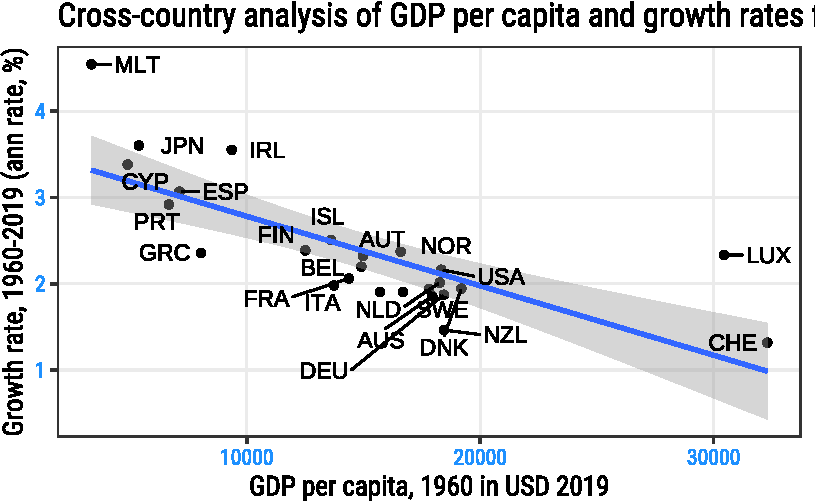
\includegraphics{01_plot_summary_files/figure-pdf/unnamed-chunk-4-1.pdf}

\subsection{}\label{section}

A trend decline in labour productivity growth sice 1960, highlighting
the UK experience within that.

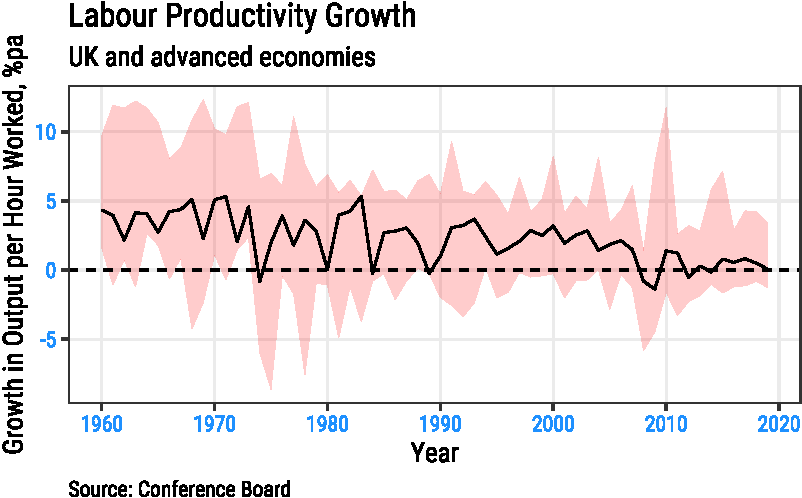
\includegraphics{01_plot_summary_files/figure-pdf/unnamed-chunk-5-1.pdf}

\subsection{Labour productivity growth and population
growth}\label{labour-productivity-growth-and-population-growth}

A raw correlation between growth in output per employed person and
population growth. Countries with higher population growth have tended,
on average, to experience lower growth in output per employed person.

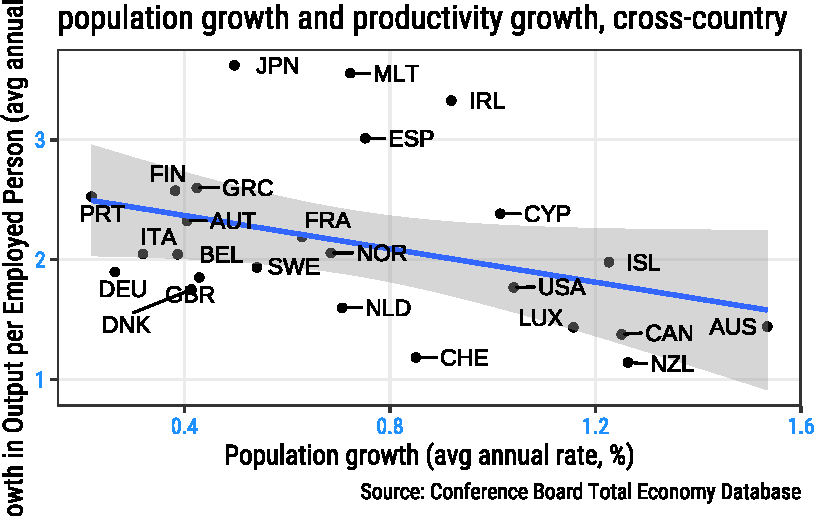
\includegraphics{01_plot_summary_files/figure-pdf/unnamed-chunk-6-1.pdf}

That association is considered a little more formally in the following
rolling regression (see Benito and Young, 2025. It shows that, across
the set of countries, the negative association between productivity and
population growth applied up until the mid-1990s, but weakened
significantly thereafter.

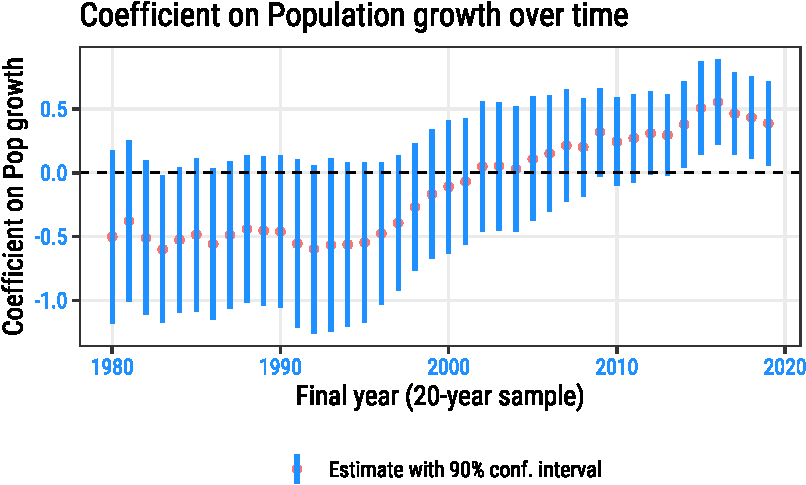
\includegraphics{01_plot_summary_files/figure-pdf/unnamed-chunk-7-1.pdf}

Has the association between productivity and population growth varied
across countries? The following suggests quite significantly so. Over
the full 1960-2019 period, the UK is one of the countries with a
significantly inverse association between these two features. By
contrast, the US stands out for having a positive association between
productivity and population growth.

That we found cross-country evidence that higher productivity growth
countries tended to have higher population growth by the end of the
period might have posed a puzzle for understanding UK experience. Our
finding that the UK has in general been in a minority of countries with
a more negative relation between its productivity growth and population
growth may help account for some of this.

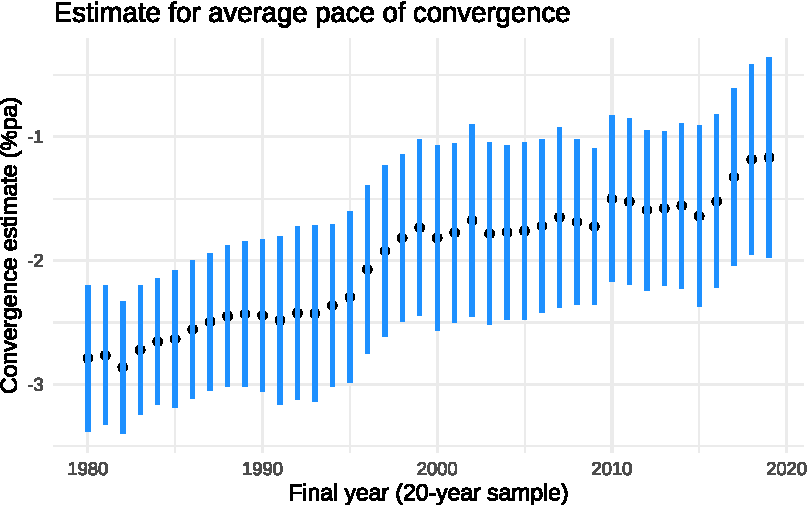
\includegraphics{01_plot_summary_files/figure-pdf/unnamed-chunk-8-1.pdf}

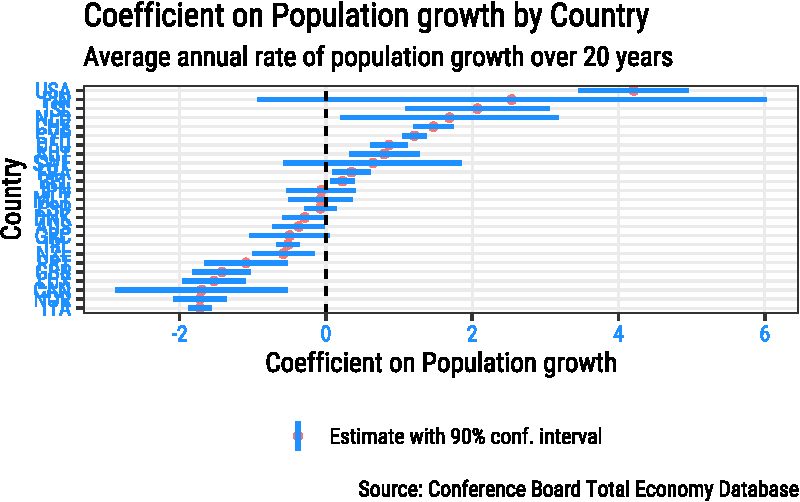
\includegraphics{01_plot_summary_files/figure-pdf/unnamed-chunk-8-2.pdf}

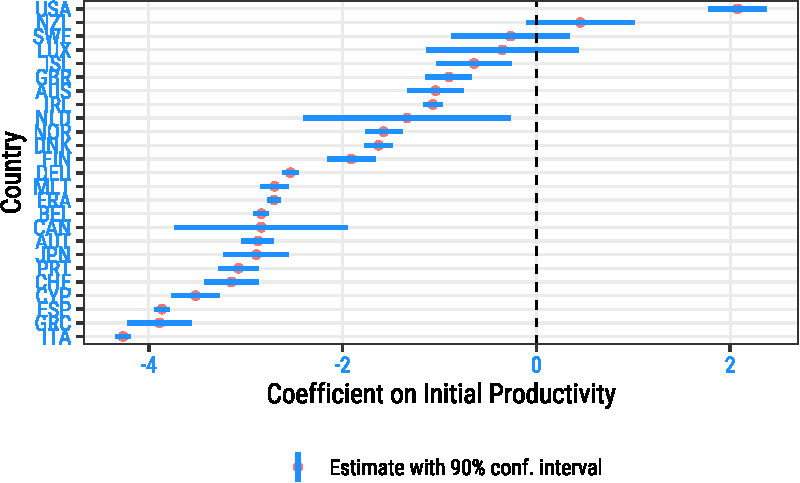
\includegraphics{01_plot_summary_files/figure-pdf/unnamed-chunk-8-3.pdf}

\subsection{Convergence}\label{convergence}

What of the UK's estimated convergence speed? Our results summarised by
the range of country-level coefficients indicate that the UK witnessed a
more modest pace of convergence, estimated at 0.90\% p.a. (standard
error = 0.14). This may also be a factor that has weighed on UK
productivity growth. Our data do not realistically allow us to explore
how these links evolved separately for each country and over time.

\subsection{Conclusions}\label{conclusions}

Our cross-country evidence together with our assessment of UK-specific
performance suggests: (i) Over time, and across countries in general,
the tendency for population growth to weigh on productivity growth that
was evident in the 1980s and 1990s has since weakened. (ii) Yet, the UK
has had a stronger tendency than most advanced economies for population
growth to go hand in hand with weaker productivity growth; (iii) a
slower pace of cross-country convergence followed the financial crisis
and may have slowed productivity growth; and (iv) slower convergence
also applies in the UK, in a feature could have owed to impaired capital
markets slowing adjustment of its capital stock to an increase in its
labour force.

The natural explanation for these findings is that there is no general
relationship between a country's productivity and population growth, as
would be consistent with long-run theory. But in the medium term, the
relationship will depend on the causes and nature of population change.
Countries at the technological frontier that have a high demand for
labour that is met partly from highly-skilled workers from the rest of
the world are likely to see faster productivity growth than countries
that experience a positive labour supply shock that is accommodated by
slow wage and productivity growth.


\printbibliography[title=References]


\end{document}
